\chapter{Eksperymenty i analiza wyników}

W rozdziale prezentuję procedurę uruchomień, zestaw parametrów i algorytmów, a następnie wyniki na grafach syntetycznych i rzeczywistych. Opis odzwierciedla stan repozytorium (skrypty w \texttt{src/glopt/cli/}) oraz zbiory wykresów w \texttt{docs/thesis/assets/figures}. Każdy wykres ma jednoznaczny podpis i interpretację, a metryki są spójne z tym, co zbiera kod.

% Na początku zostały opisane kryteria oceny, które określają sposób interpretacji wyników. Każda z metryk ma swoje znaczenie praktyczne – część z nich odnosi się do wartości absolutnych, takich jak koszt rozwiązania czy czas działania algorytmu, a część ma charakter względny, umożliwiający porównania między algorytmami i odniesienie ich jakości do rozwiązań optymalnych uzyskanych za pomocą ILP. Dzięki temu możliwe było równoczesne ujęcie wyników w dwóch wymiarach: faktycznego kosztu i czasu obliczeń oraz dystansu od optimum.

% Następnie zostało opisane środowisko testowe, w którym przeprowadzono eksperymenty. Uwzględniono zarówno parametry sprzętowe i programowe, jak i narzędzia wykorzystane do implementacji i analizy. Osobną uwagę poświęcono grafom testowym. W przypadku grafów syntetycznych wzięto pod uwagę trzy klasy: losowe (\textit{random}), bezskalowe (\textit{scale-free}) oraz typu małego świata (\textit{small-world}). Dla każdej klasy przygotowano serie instancji o rosnącej liczbie wierzchołków. Zakresy były różne: grafy losowe analizowano od 10 do 90 węzłów, grafy small-world do 230 węzłów, natomiast grafy bezskalowe do 990 węzłów. Wartości te rosły co 20 węzłów, co pozwoliło na obserwację zmian jakości i czasu działania algorytmów w funkcji rozmiaru problemu. Zróżnicowanie maksymalnych rozmiarów wynikało z charakteru samych grafów – grafy losowe i small-world szybciej prowadziły do długich czasów obliczeń przy większych rozmiarach, natomiast grafy scale-free pozwalały na analizę znacznie większych instancji. Oprócz grafów syntetycznych wykorzystano także grafy rzeczywiste, które uzupełniają analizę o przykłady praktycznych struktur sieciowych.

% Najobszerniejszą część rozdziału stanowi opis eksperymentów i ich wyników. Wyniki zostały przedstawione osobno dla grafów syntetycznych i rzeczywistych, a w każdym przypadku uwzględniono zarówno wartości średnie, jak i ich odniesienia do najlepszych wyników. W przypadku grafów syntetycznych zwrócono uwagę na różnice pomiędzy poszczególnymi klasami grafów oraz na zależność jakości i czasu od rosnącej liczby węzłów. W przypadku grafów rzeczywistych omówiono trzy zestawy instancji, podkreślając odmienny charakter danych oraz wpływ tej różnorodności na zachowanie algorytmów. We wszystkich analizach kluczową rolę odegrały porównania względem ILP, które pełniło funkcję punktu odniesienia dla jakości rozwiązań.

% W końcowej części rozdziału została przeprowadzona analiza wpływu parametrów algorytmów na ich skuteczność. Uwzględniono między innymi temperaturę początkową i tempo chłodzenia w przypadku symulowanego wyżarzania, a także parametry sterujące intensywnością przeszukiwania w metodach tabu search czy ant colony optimization. Analiza ta pokazała, w jakim stopniu dobrane ustawienia wpływają na kompromis między jakością a czasem działania algorytmu oraz które wartości parametrów pozwalają uzyskać najbardziej stabilne i korzystne rezultaty.

\section{Kryteria oceny}

Wszystkie skrypty zapisują spójne metryki (koszt, czas, poprawność oraz statystyki grup), na których opieram wykresy i porównania. Kluczowe pola w CSV:

\begin{itemize}
    \item \textbf{cost\_per\_node} \\
    Koszt znormalizowany przez liczbę węzłów — umożliwia porównywanie instancji o różnych rozmiarach oraz różnych rodzinach grafów.

    \item \textbf{time\_ms} \\
    Czas obliczeń jednej próby (ms), mierzony ścienny — praktyczny koszt obliczeniowy metody.

    \item \textbf{total\_cost} \\
    Wartość funkcji celu — jakość rozwiązania. W agregacjach odnoszę ją do najmniejszej wartości uzyskanej w danej rodzinie (lub do ILP, jeśli jest dostępne).

    \item \textbf{valid}, \textbf{issues} \\
    Poprawność rozwiązania i liczba naruszeń (gdyby wystąpiły) raportowane przez walidator.

    \item \textbf{średni koszt ILP (mean\_ilp\_cost)} \\
    Wartość optymalna kosztu, uzyskana z rozwiązania za pomocą programowania całkowitoliczbowego (ILP). 
    Stanowi punkt odniesienia dla pozostałych algorytmów – na jego podstawie liczone są wskaźniki jakości (mean\_cost\_ratio). 
    Dzięki temu możliwe jest obiektywne porównanie heurystyk.

    \item \textbf{średni czas ILP (mean\_ilp\_time)} \\
    Uśredniony czas rozwiązania problemu metodą ILP. 
    Pokazuje koszt obliczeniowy uzyskania optimum i pozwala zestawić go z czasem uzyskanym przy użyciu innego algorytmu. 
    W praktyce często jest istotny, bo wskazuje, że choć ILP daje rozwiązanie optymalne, 
    to bywa obliczeniowo niepraktyczne dla dużych instancji.

    \item \textbf{liczność próby (count)} \\
    Liczba instancji, na podstawie których obliczono średnie wartości metryk. 
    Duża liczność zwiększa wiarygodność uśrednień, a mała liczność oznacza, 
    że wyniki mogą być mniej reprezentatywne. 
\end{itemize}

\section{Środowisko i uruchamianie}
Wszystkie eksperymenty uruchamiam w Pythonie 3.13 - wersja jest wymuszona w projekcie i sprawdzana na starcie. Do zarządzania środowiskiem używam narzędzia \texttt{uv}. W repozytorium mam prosty \texttt{Makefile}, który odpala skrypty CLI bez dodatkowych parametrów. To było dla mnie wygodne, bo cała konfiguracja leży na górze plików w folderze \texttt{src/glopt/cli/} i mogę to łatwo zmieniać w kodzie bez długich parserów linii poleceń. Każdy skrypt na starcie drukuje w logu najważniejsze ustawienia, potem raportuje postęp w pętlach i na koniec robi krótkie podsumowanie. Logi zapisują się do \texttt{runs/<run\_id>/glopt.log} i jednocześnie lecą na konsolę.

Zestaw \texttt{benchmark\_all} to grafy syntetyczne - trzy rodziny. Zestaw \texttt{benchmark\_real\_all} to ego-sieci Facebooka. Po uruchomieniu \texttt{make analyze-csv} z odpowiednim CSV powstaje folder \texttt{results/...} z wykresami i tabelami. Mam też skrypt, który kopiuje wybrane PNG do katalogu pracy: \texttt{make thesis-figs} - dzięki temu figury są w \texttt{docs/thesis/assets/figures} i mogę je wprost wstawić do rozdziału.

\subsection*{Konfiguracja sprzętowo-programowa}
\begin{itemize}
  \item System: Ubuntu 24.04 LTS (WSL2), CPU Intel Core i5-14600KF (16 wątków), RAM~24~GiB (dla WSL2).
  \item Środowisko: Python~3.13, biblioteki: networkx, pulp (CBC), numpy, pandas, matplotlib.
  \item Czas: wszystkie czasy to średnie z wielu powtórzeń (patrz \S\,Organizacja eksperymentów), z limitem czasu dla ILP.
\end{itemize}

\subsection*{Parametry algorytmów}
\begin{table}[h]
\centering
\begin{tabular}{@{}ll@{}}
\toprule
Algorytm & Parametry (wartości domyślne) \\
\midrule
Greedy & kolejność wg stopnia/efektywności licencji \\
Genetic & populacja=30, generacje=40, elita=20\%, crossover=0.6 \\
Simulated Annealing & $T_0$ dobrane eksperymentalnie, ochładzanie geometr. \\
Tabu Search & tabu tenure ok.~20, sąsiedztwo mutacji grup \\
Ant Colony & $\alpha=1,\beta=2$, parowanie=0.5, $q_0=0.9$, 20 mrówek \\
ILP & CBC, limit czasu na instancję \\
\bottomrule
\end{tabular}
\caption{Zestawienie głównych parametrów algorytmów użytych w eksperymentach.}
\label{tab:algo_params}
\end{table}

\section{Wybrane wykresy - grafy syntetyczne}
Na rysunkach poniżej pokazuję kilka reprezentatywnych figur (pełny komplet wykresów i tabel znajduje się w katalogu wyników). Odwołania w tekście używają etykiet \ref{fig:random_duo_cost_time}–\ref{fig:ilp_timeout}.

\begin{figure}[h]
  \centering
  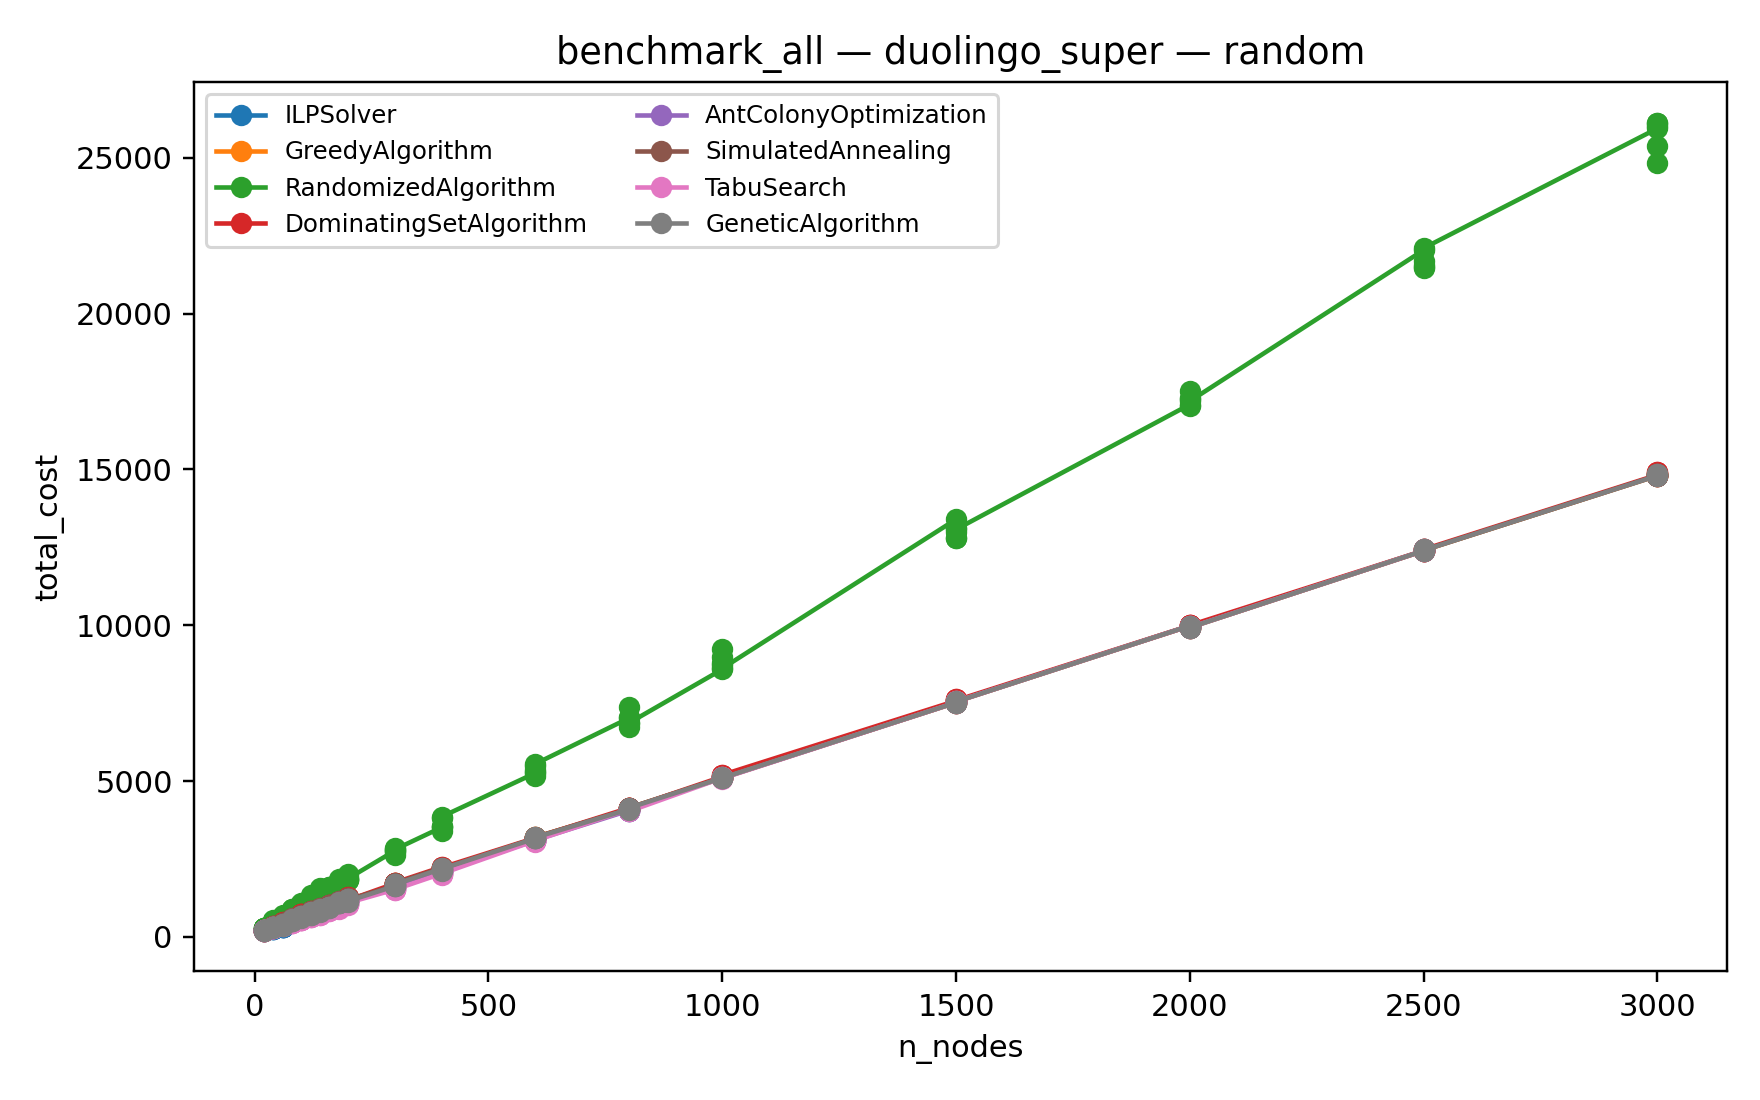
\includegraphics[width=0.48\linewidth]{assets/figures/ba_random_duo_cost_vs_n.png}
  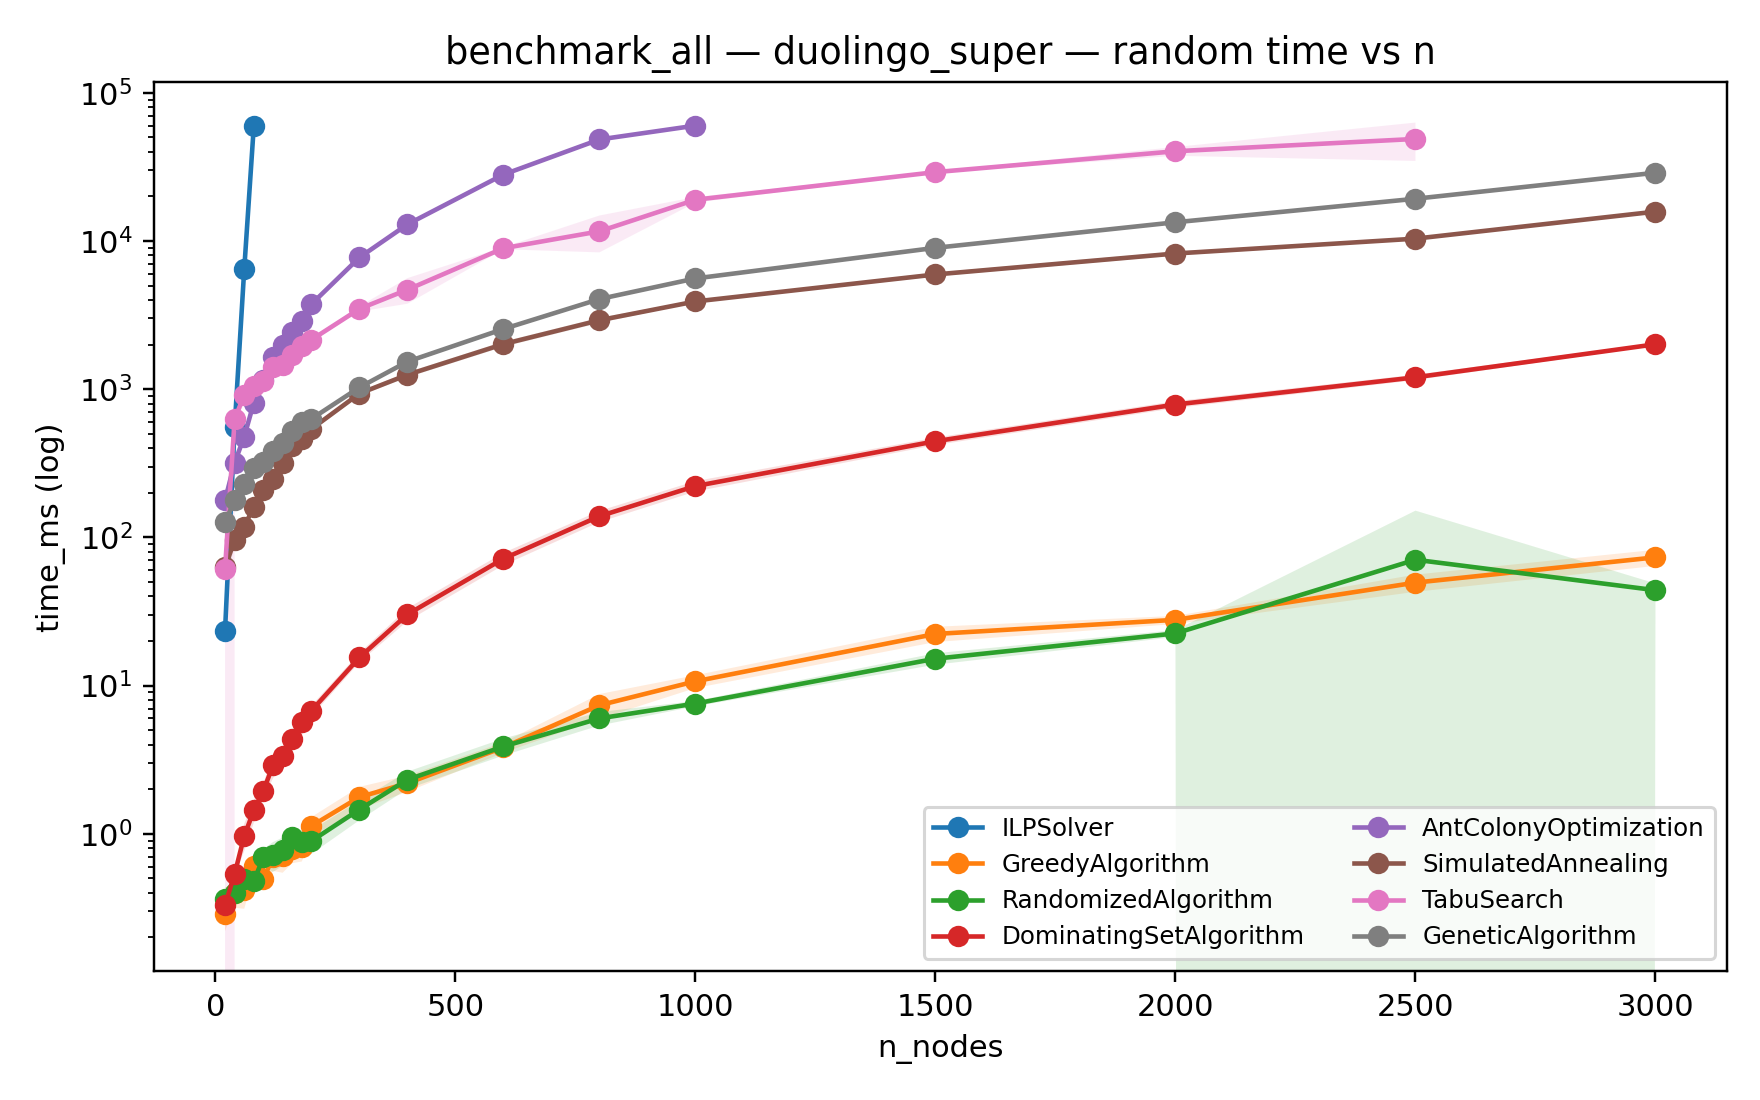
\includegraphics[width=0.48\linewidth]{assets/figures/ba_random_duo_time_vs_n.png}
  \caption{Random - Duolingo Super - koszt i czas w funkcji n.}
  \label{fig:random_duo_cost_time}
\end{figure}

\begin{figure}[h]
  \centering
  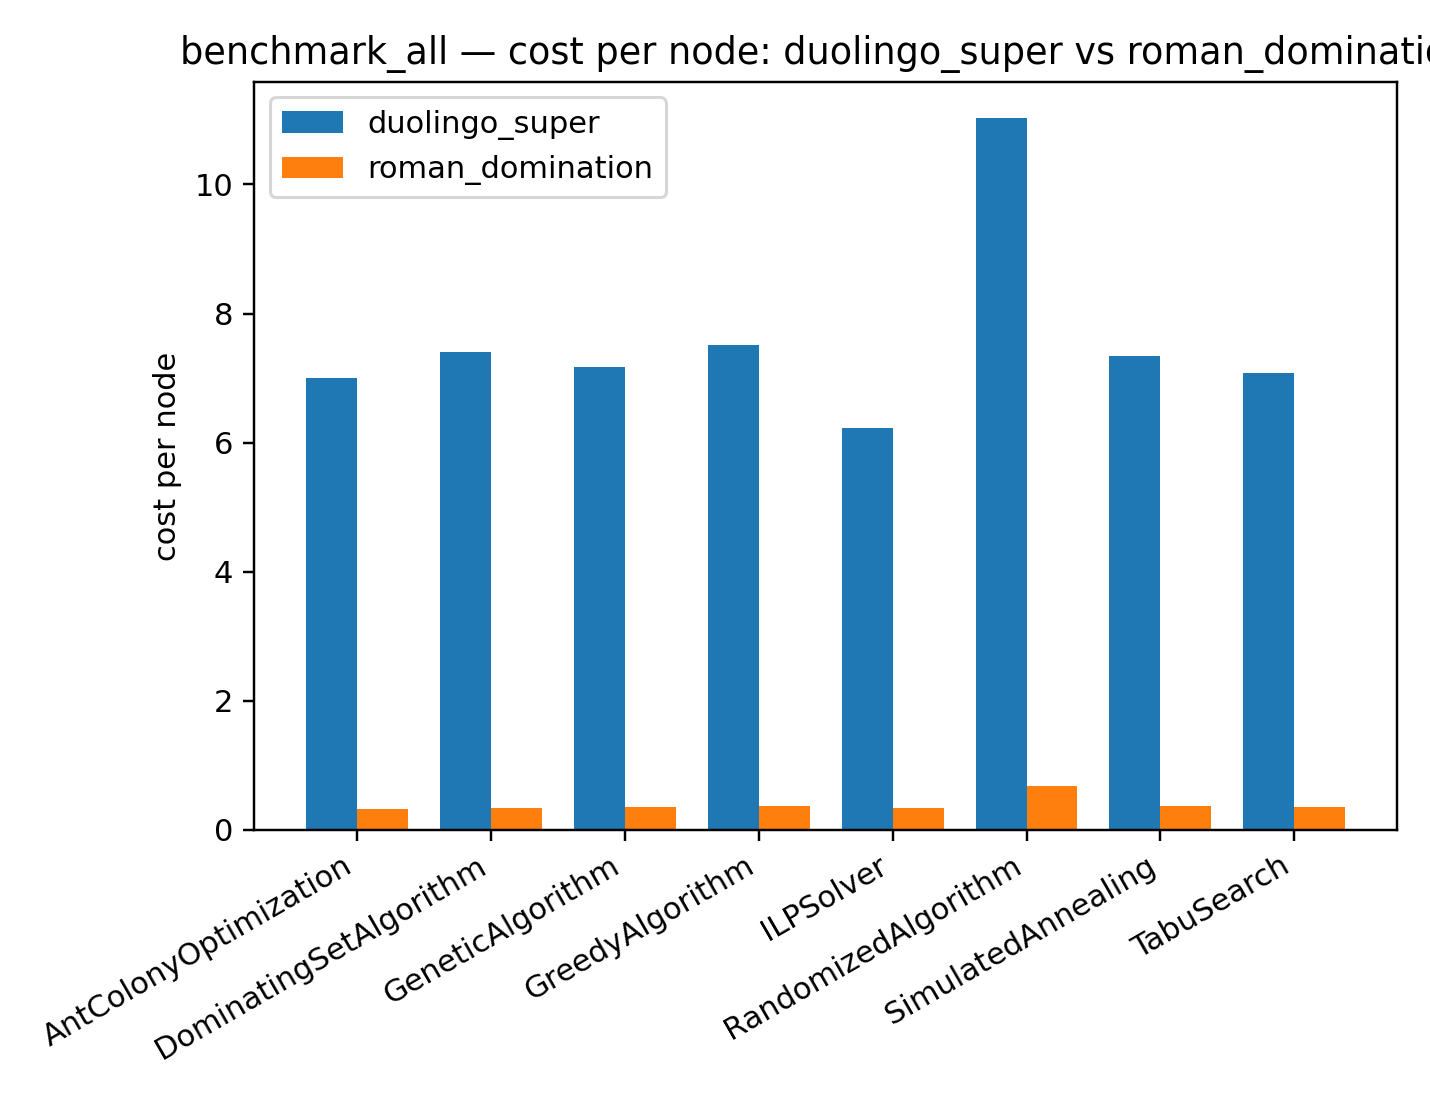
\includegraphics[width=0.48\linewidth]{assets/figures/ba_compare_cost_duo_vs_roman.png}
  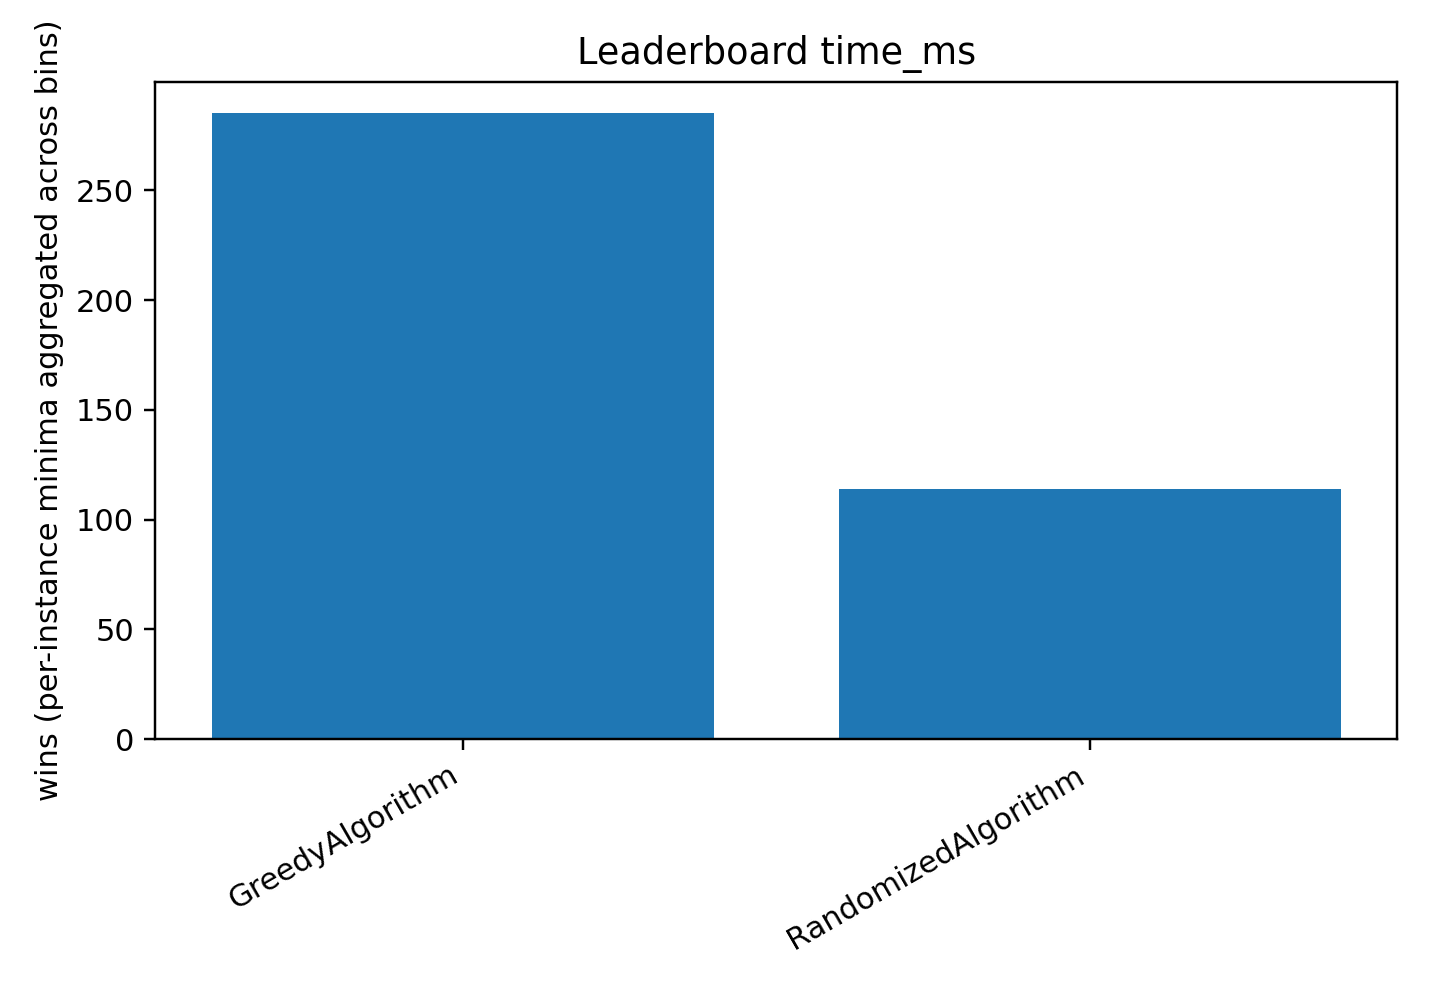
\includegraphics[width=0.48\linewidth]{assets/figures/ba_leaderboard_time.png}
  \caption{Porównanie konfiguracji licencji - koszt na węzeł oraz „leaderboard” czasu.}
  \label{fig:compare_duo_roman}
\end{figure}

\begin{figure}[h]
  \centering
  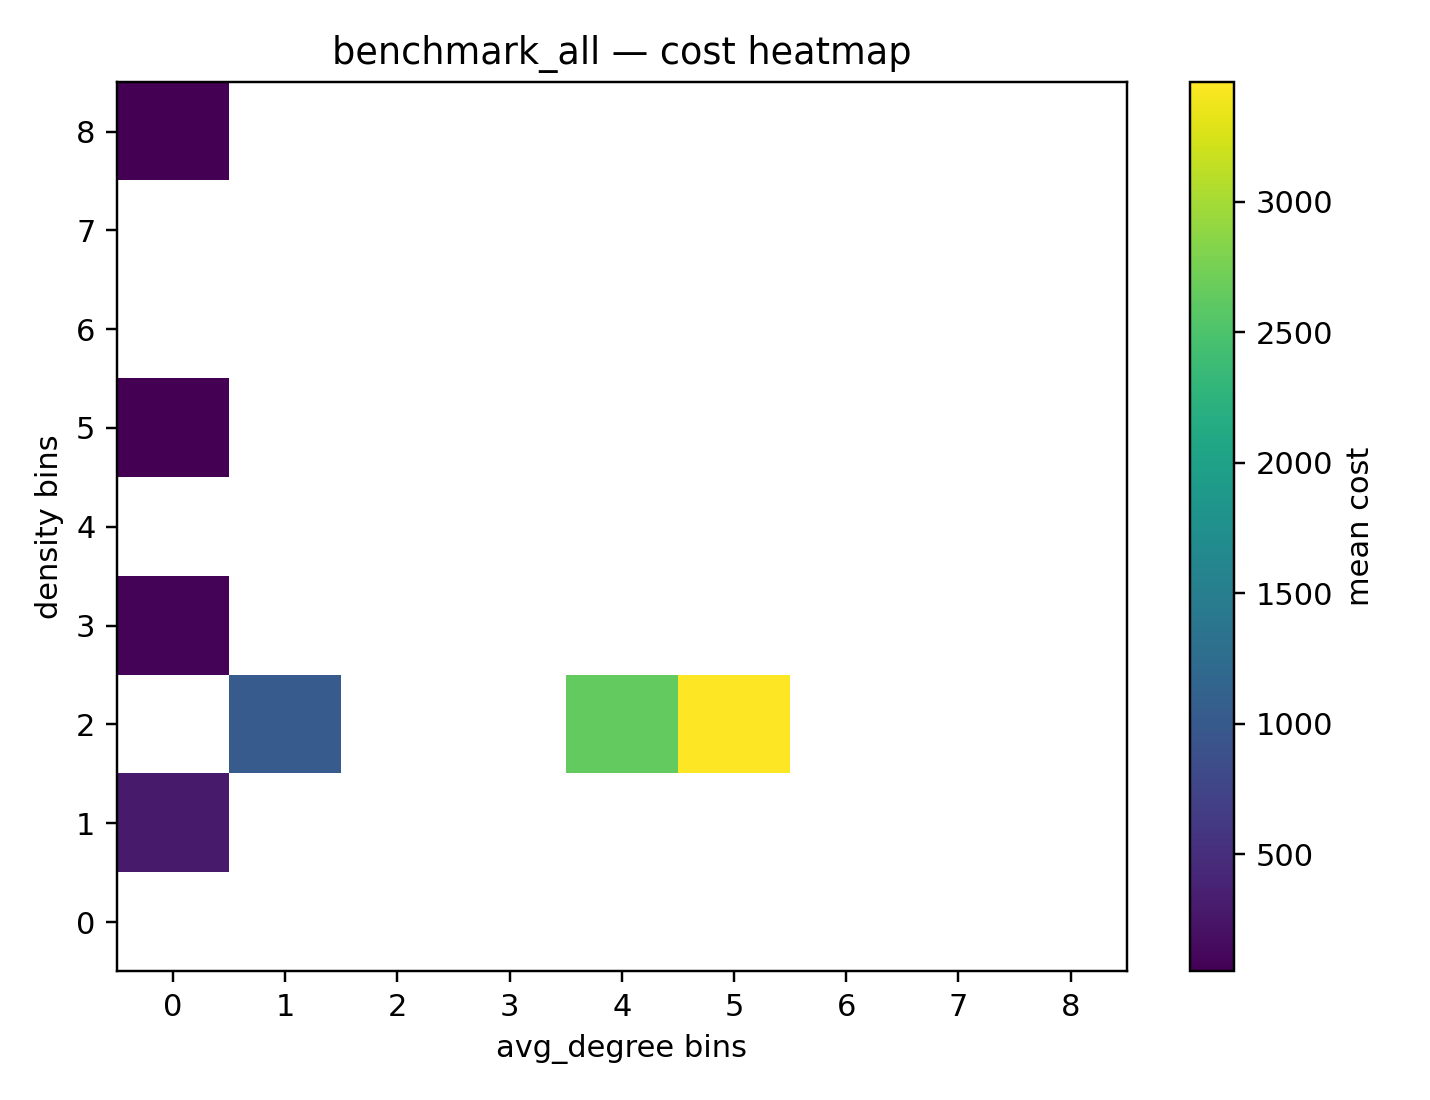
\includegraphics[width=0.6\linewidth]{assets/figures/ba_heatmap_cost.png}
  \caption{Heatmapa średniego kosztu względem gęstości i średniego stopnia.}
  \label{fig:heatmap_cost}
\end{figure}

W skrócie: algorytmy zachłanne i proste losowe są bardzo szybkie i dają akceptowalną jakość; metaheurystyki (GA/SA/TS/ACO) schodzą niżej kosztowo, kosztem czasu obliczeń. ILP jest punktem odniesienia dla małych $n$, a następnie szybko napotyka limity czasu (por. rys.\,\ref{fig:ilp_timeout}).

\section{Wybrane wykresy - grafy rzeczywiste}
Analogiczne obserwacje dotyczą ego-sieci Facebooka (rys.\,\ref{fig:facebook_ego_cost}–\ref{fig:facebook_compare_cost}).

\begin{figure}[h]
  \centering
  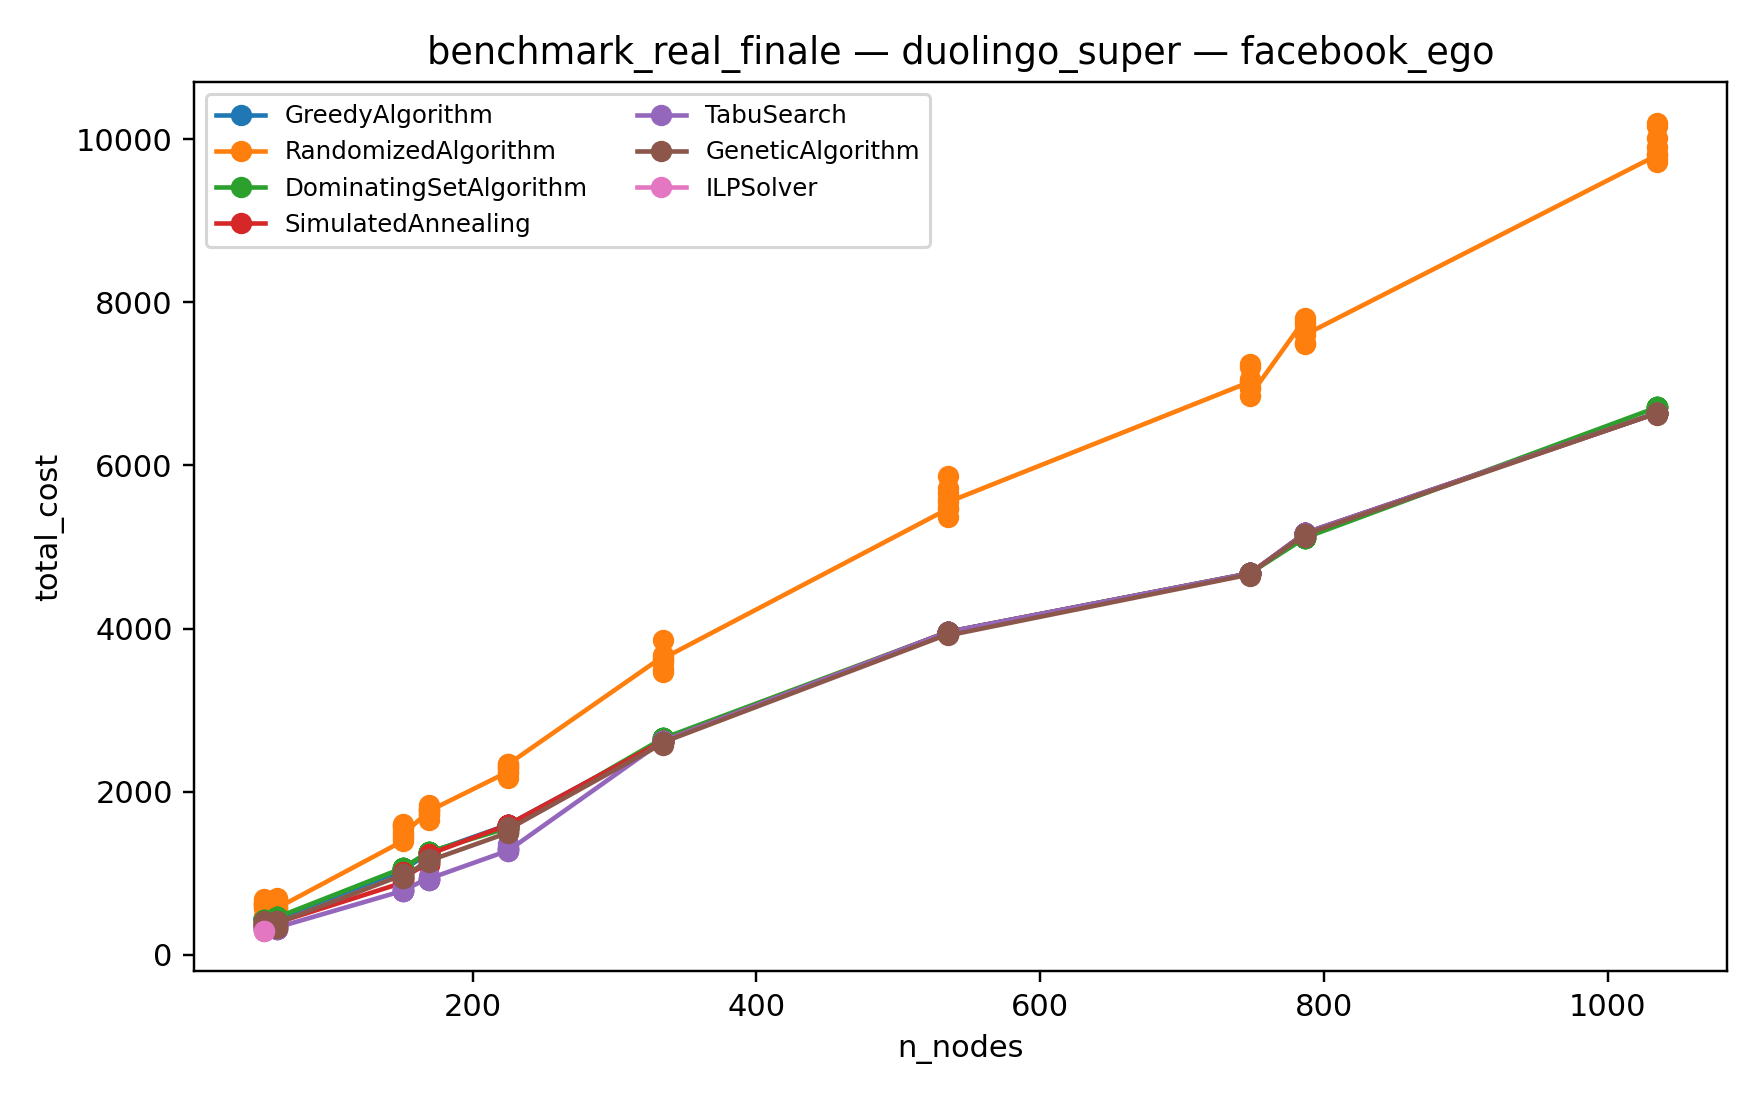
\includegraphics[width=0.48\linewidth]{assets/figures/br_facebook_ego_duo_cost_vs_n.png}
  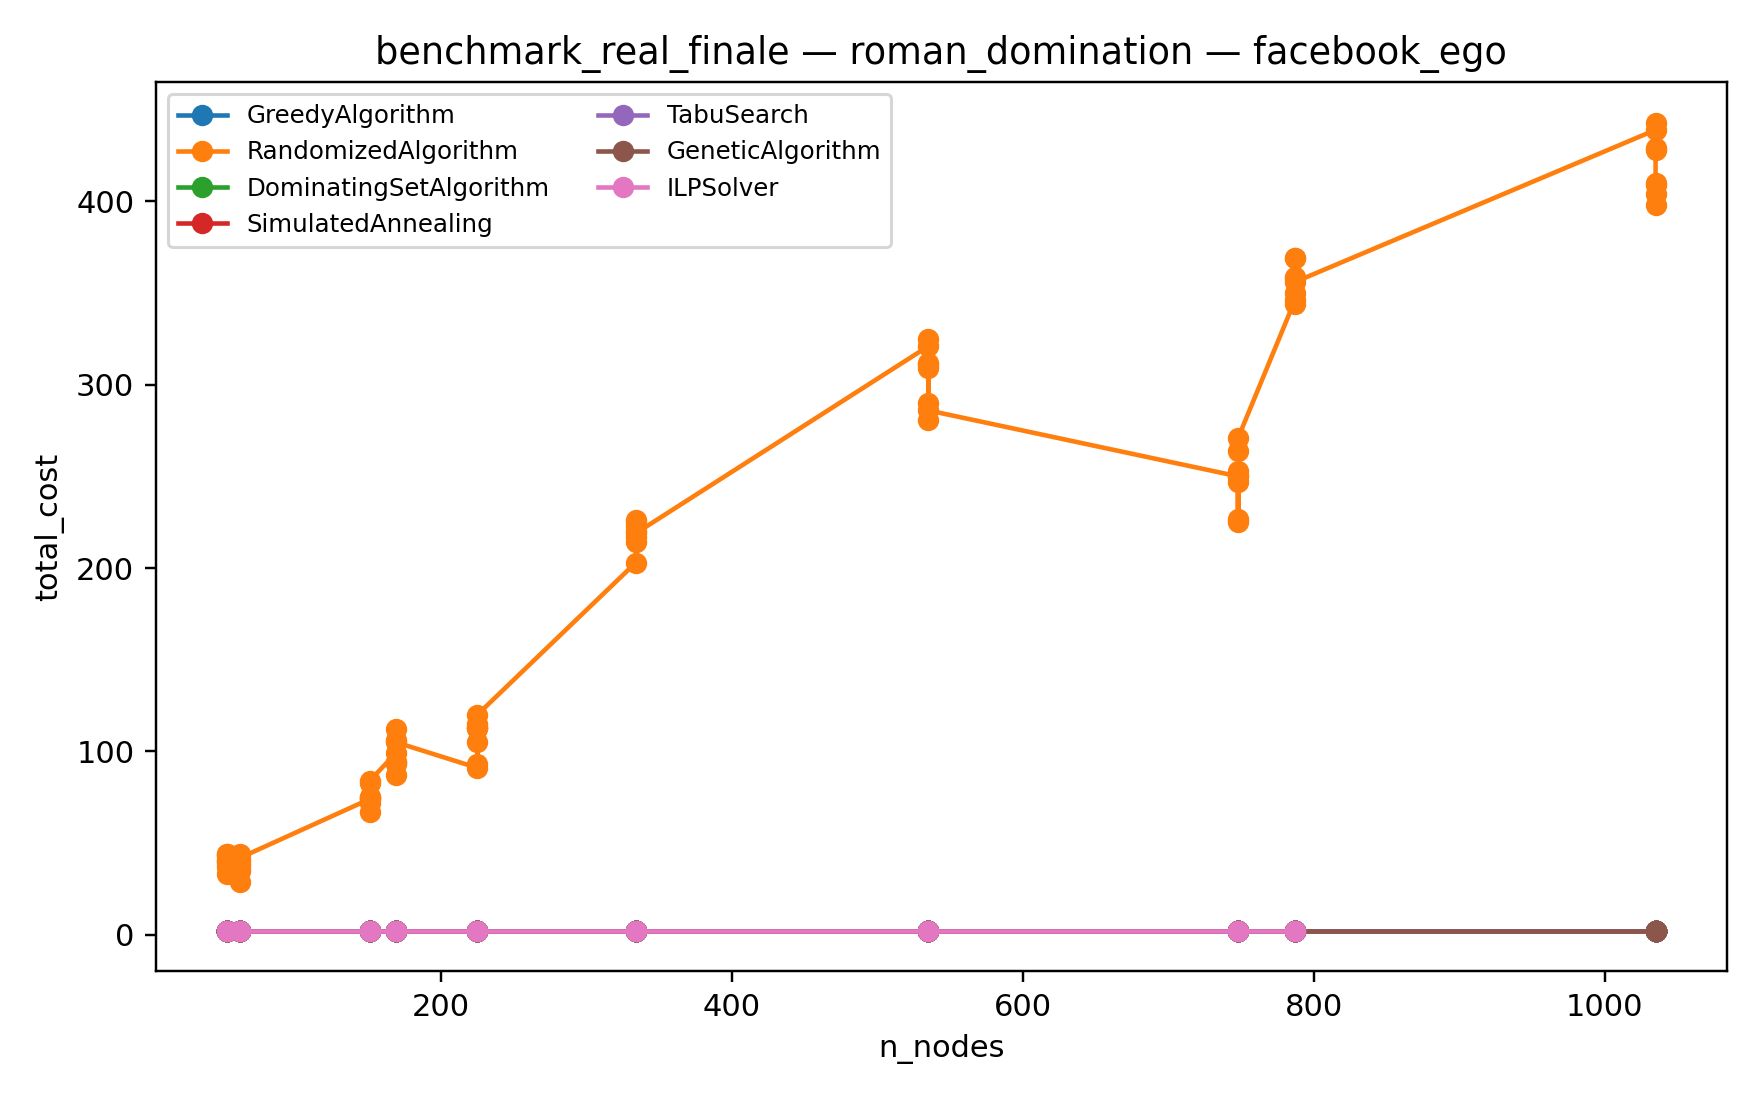
\includegraphics[width=0.48\linewidth]{assets/figures/br_facebook_ego_roman_cost_vs_n.png}
  \caption{Facebook ego - koszt w funkcji n dla Duolingo Super i Roman domination.}
  \label{fig:facebook_ego_cost}
\end{figure}

\begin{figure}[h]
  \centering
  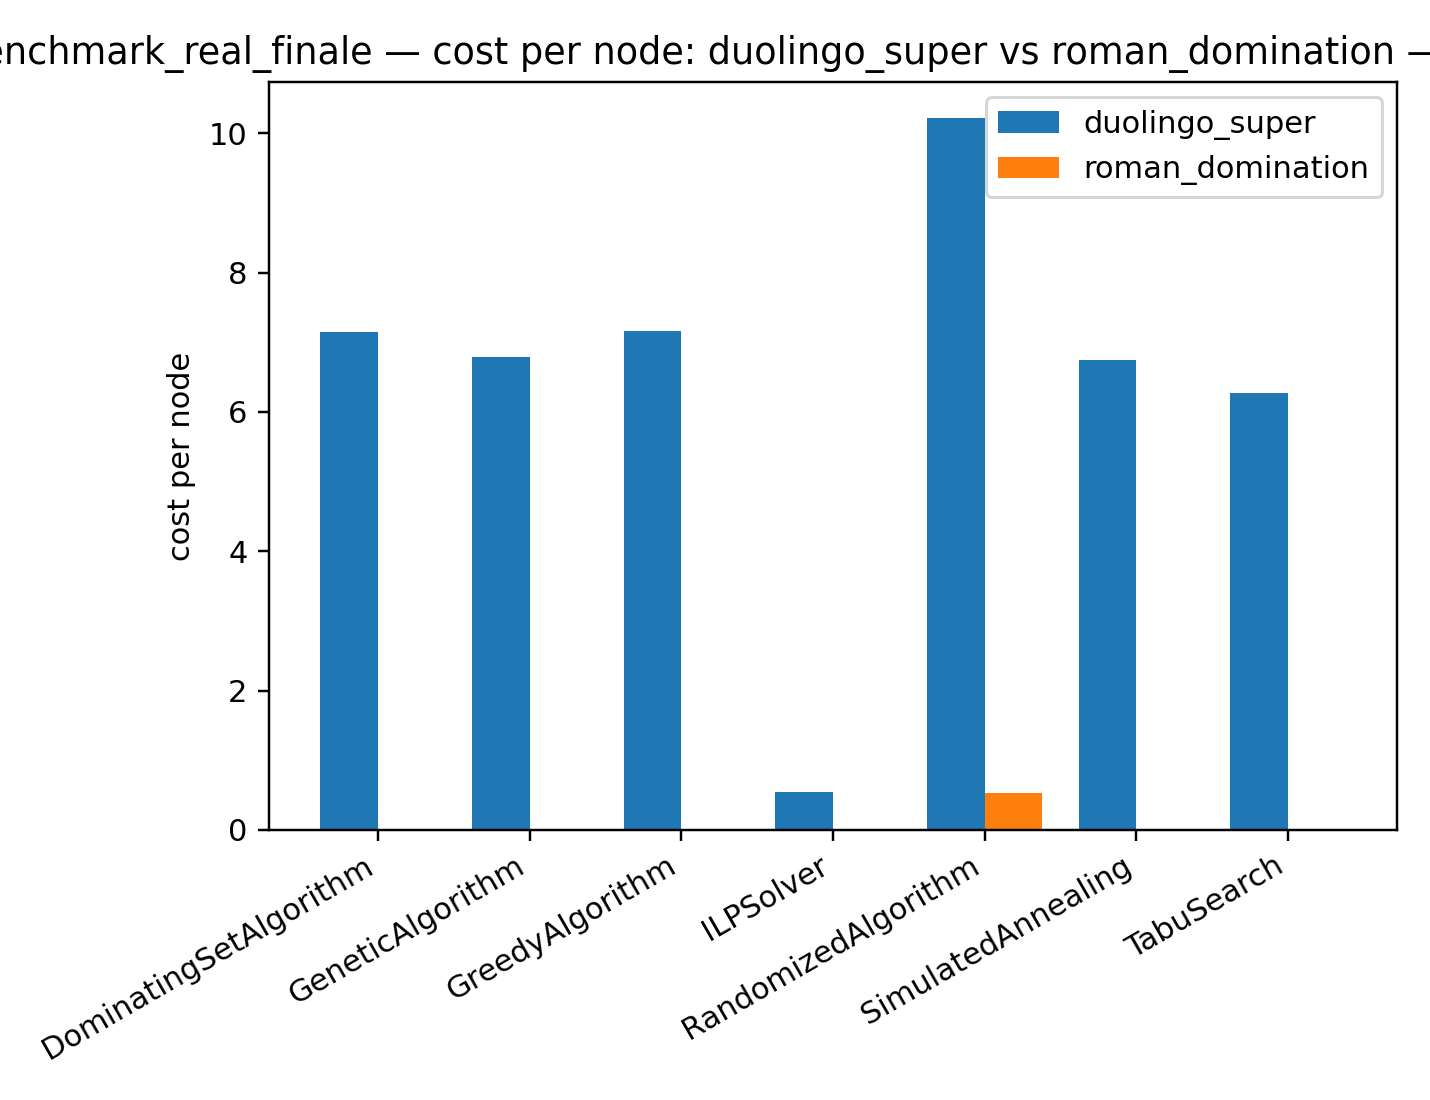
\includegraphics[width=0.48\linewidth]{assets/figures/br_compare_cost_duo_vs_roman_facebook_ego.png}
  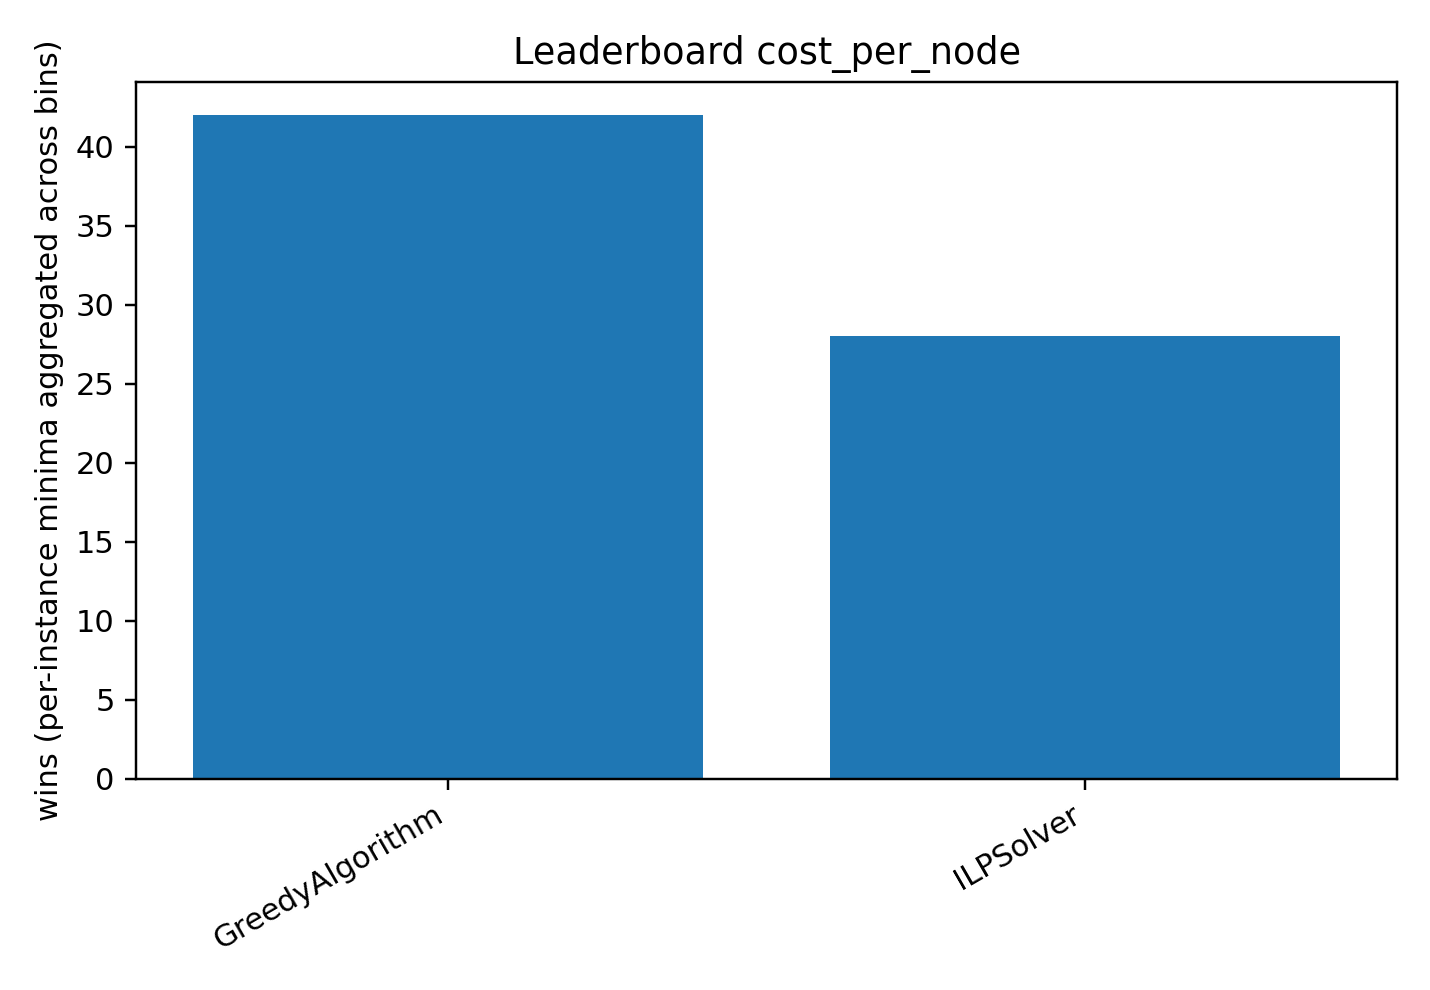
\includegraphics[width=0.48\linewidth]{assets/figures/br_leaderboard_cost.png}
  \caption{Porównanie konfiguracji licencji na facebook\_ego oraz leaderboard kosztu.}
  \label{fig:facebook_compare_cost}
\end{figure}

W praktyce duolingo\_super i roman\_domination to dwa najważniejsze zestawy - te porównania są głównym punktem odniesienia w wnioskach końcowych.

\section{Granica wykonalności ILP}
Na małych instancjach ILP daje nam złoty punkt odniesienia. Potem szybko pojawia się granica, gdzie solver zaczyna przekraczać limity czasu. Na rysunkach poniżej pokazuję prosty obraz tej granicy: heatmapa udziału timeoutów w siatce gęstość kontra rozmiar n oraz chmura punktów sukces kontra timeout.

\begin{figure}[h]
  \centering
  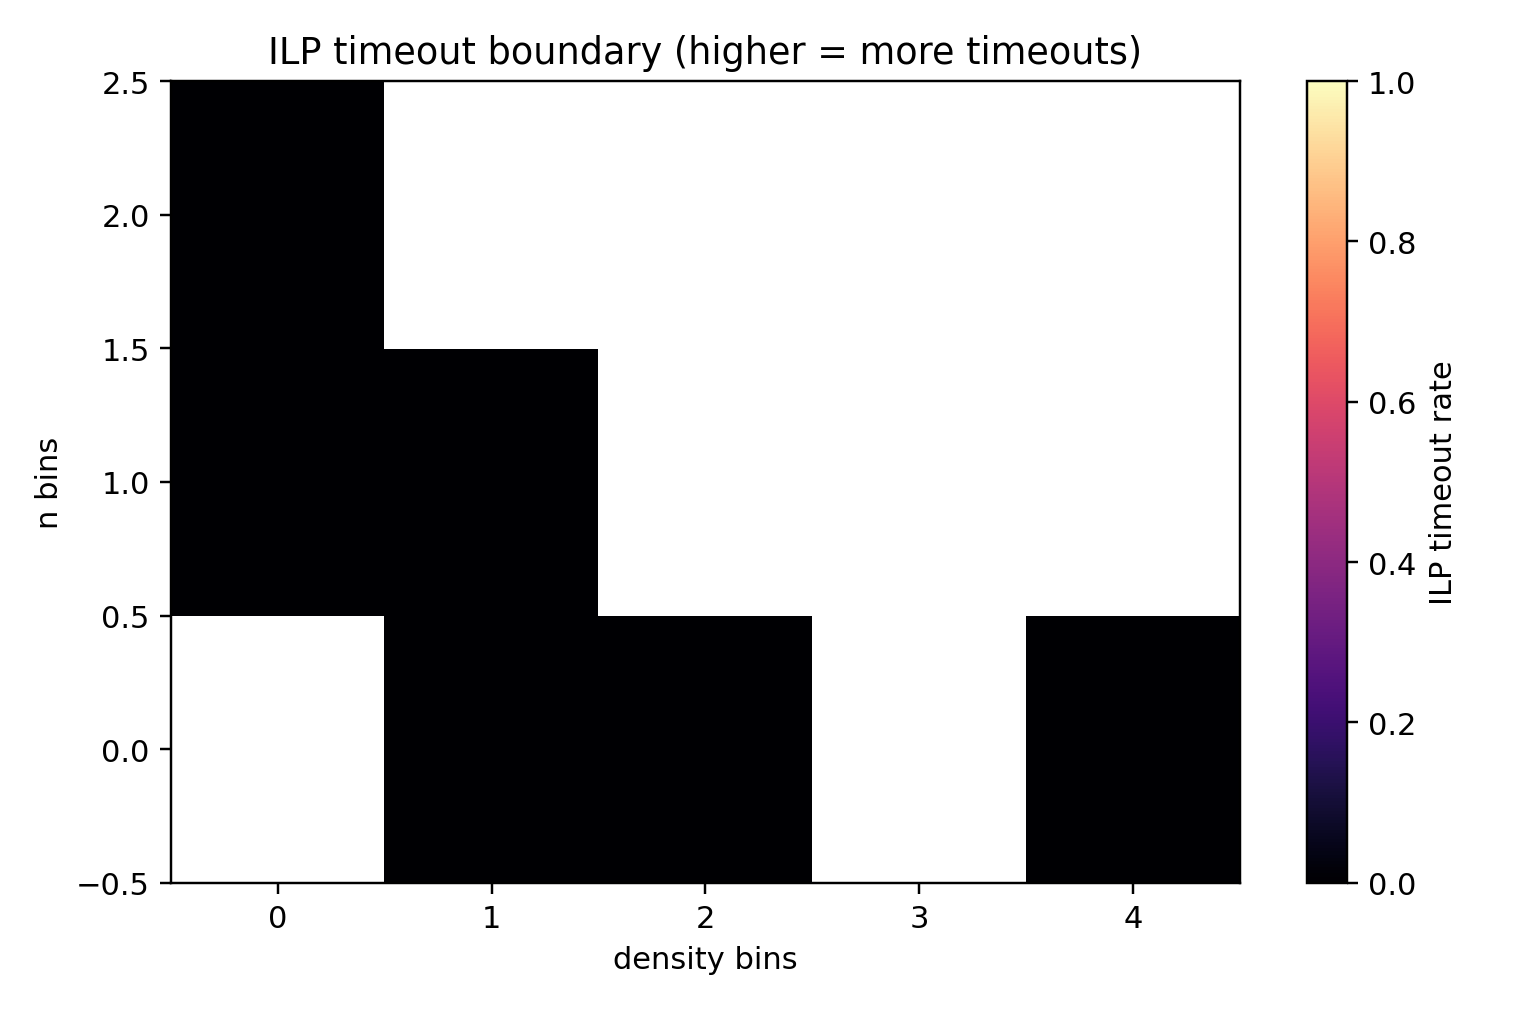
\includegraphics[width=0.48\linewidth]{assets/figures/ba_ilp_timeout_boundary.png}
  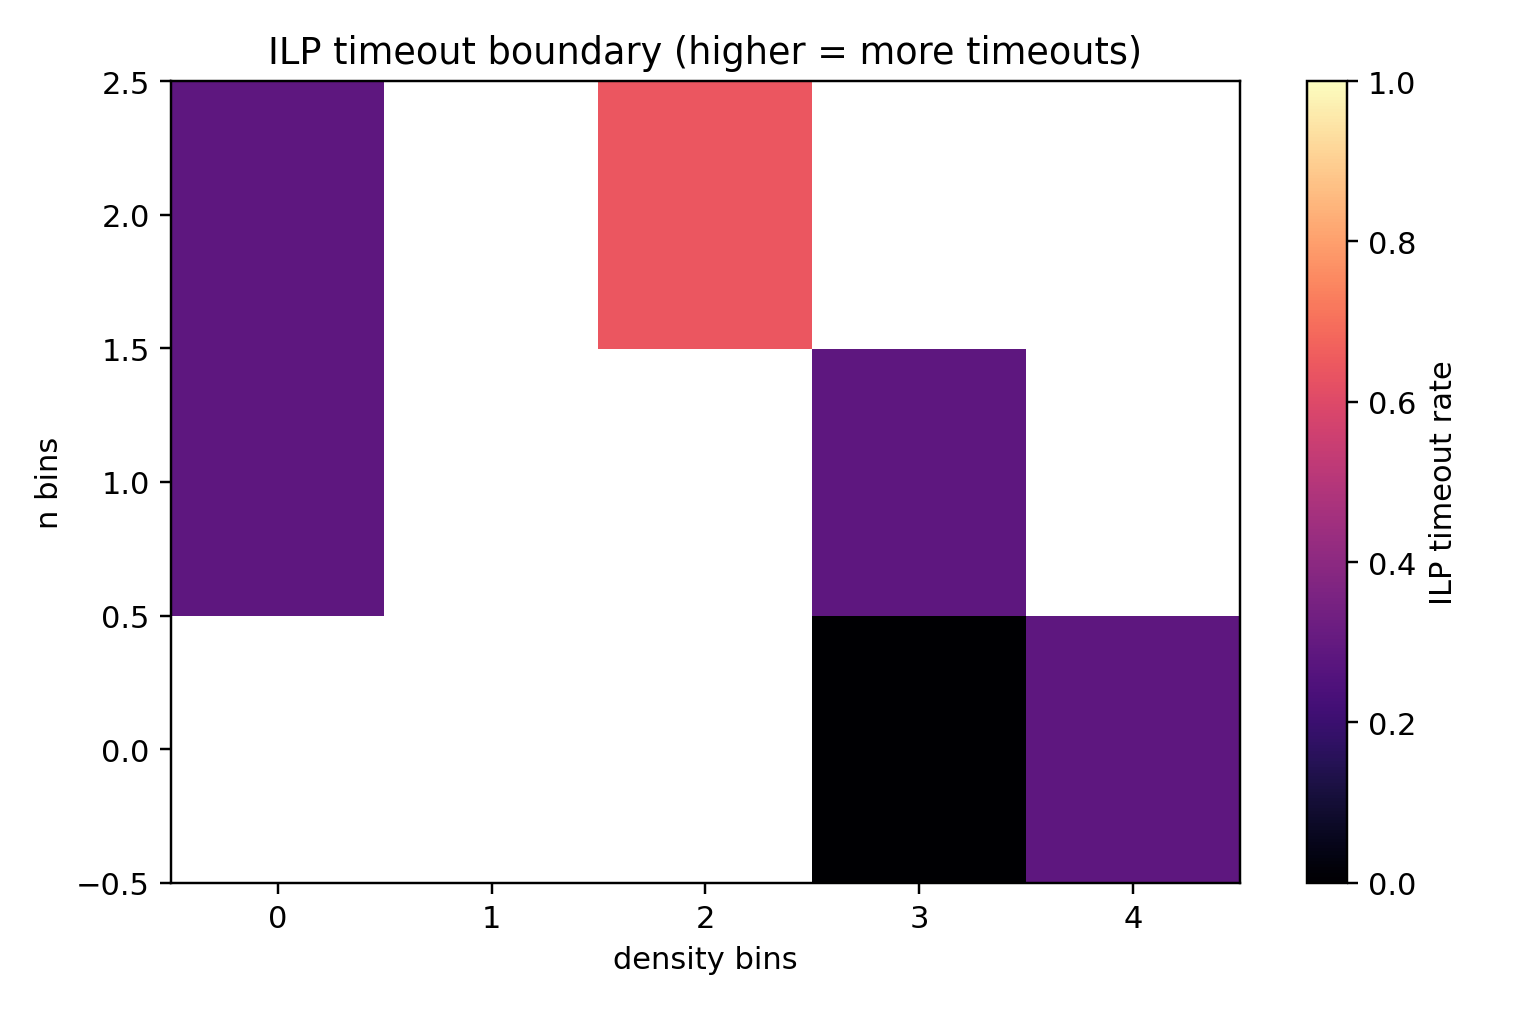
\includegraphics[width=0.48\linewidth]{assets/figures/br_ilp_timeout_boundary.png}
  \caption{Granica czasowa ILP: po lewej grafy syntetyczne, po prawej grafy rzeczywiste (jaśniejsze = więcej timeoutów).}
  \label{fig:ilp_timeout}
\end{figure}

Widać, że wraz ze wzrostem n i gęstości rośnie procent timeoutów. To potwierdza praktyczną rolę ILP jako algorytmu referencyjnego do mniejszych zadań i motywuje użycie heurystyk oraz metaheurystyk dla większych sieci.


\section{Środowisko testowe}

W celu zapewnienia powtarzalności badań oraz wyjaśnienia potencjalnego wpływu konfiguracji sprzętowej i programowej na uzyskane wyniki przedstawiono poniżej szczegóły dotyczące środowiska w którym były on przeprowadzane.

\subsection{Konfiguracja sprzętowa}
\begin{itemize}
    \item Procesor: 
    \item Pamięć RAM: 
    \item Dysk: 
    \item System operacyjny: 
\end{itemize}

\subsection{Środowisko programistyczne}

Do implementacji oraz analizy wykorzystano język Python wraz z kilkoma kluczowymi bibliotekami:

\begin{itemize}
    \item \texttt{networkx} – biblioteka przeznaczona do tworzenia, manipulacji i analizy struktur grafowych. 
    W eksperymentach posłużyła jako główne narzędzie do reprezentacji instancji problemu. 
    Dzięki niej możliwe było zarówno generowanie grafów syntetycznych, 
    jak i wczytywanie oraz przetwarzanie grafów rzeczywistych. 
    Udostępnia również podstawowe algorytmy pomocnicze oraz narzędzia do analizy własności strukturalnych, 
    co pozwoliło zweryfikować poprawność przygotowanych instancji.

    \item \texttt{numpy} oraz \texttt{pandas} – podstawowe narzędzia do pracy z danymi numerycznymi i tabelarycznymi. 
    Biblioteka \texttt{numpy} zapewnia wydajne operacje macierzowe i wektorowe, co było przydatne w obliczeniach wykonywanych w pętli podczas działania algorytmów. 
    Natomiast \texttt{pandas} umożliwiło uporządkowane przechowywanie wyników w strukturach \texttt{DataFrame}, 
    ich łatwe filtrowanie, agregowanie i eksport do formatu \texttt{Excel}, 
    na podstawie którego przygotowano dalsze analizy i wizualizacje. 
    Te dwie biblioteki stanowiły podstawę całego procesu gromadzenia i przetwarzania danych.

    % \item \texttt{matplotlib} – biblioteka do tworzenia wizualizacji, 
    % wykorzystana do generowania wykresów prezentujących wyniki eksperymentów. 
    % Z jej pomocą powstały zarówno podstawowe wykresy liniowe, jak i bardziej złożone zestawienia porównawcze, 
    % które zostały następnie przeniesione do arkuszy kalkulacyjnych i posłużyły do ostatecznej interpretacji wyników. 
    % Dzięki \texttt{matplotlib} możliwe było szybkie prototypowanie wizualizacji i sprawdzanie trendów 
    % jeszcze na etapie weryfikacji poprawności obliczeń.
\end{itemize}


\subsection{Charakterystyka grafów testowych}

\textbf{Syntetyczne.} Trzy rodziny: \textit{random} (Erdős–Rényi, $p=0{.}10$), \textit{small-world} (Watts–Strogatz, $k=6$, $p=0{.}05$, $k$ wymuszane parzyste) i \textit{scale-free} (Barabási–Albert, $m=2$). Rozmiary: \(n\in\{20,40,\dots,200\}\) i \(n\in\{300,400,600,800,1000,1500,2000,2500,3000\}\). Na każdy punkt: \(\texttt{SAMPLES\_PER\_SIZE}=3\) próbek i \(\texttt{REPEATS\_PER\_GRAPH}=2\).

\textbf{Rzeczywiste.} Ego-sieci Facebooka (SNAP), bez parametrycznego sterowania rozmiarem; raportuję \(|V|,|E|\), gęstość, średni stopień, klasteryzację i liczbę składowych.


\subsection{Organizacja eksperymentów i uruchomienia}\label{subsec:uruchomienia}
Uruchomienia są skryptowe i powtarzalne:
\begin{itemize}
  \item \textbf{Syntetyczne (statyczne):} \texttt{src/glopt/cli/benchmark.py}. Rodziny, rozmiary i powtórzenia jak wyżej; twardy limit czasu \(60\,\mathrm{s}\) na próbę (zabicie procesu potomnego), co wyznacza granicę wykonalności ILP.
  \item \textbf{Rzeczywiste (statyczne):} \texttt{src/glopt/cli/benchmark\_real.py}. Ego-sieci Facebooka; analogiczne metryki i limit \(60\,\mathrm{s}\).
  \item \textbf{Syntetyczne (dynamiczne):} \texttt{src/glopt/cli/dynamic.py}. Każdy bazowy graf ewoluuje przez \(\texttt{NUM\_STEPS}=50\) kroków zgodnie z parametrami mutacji: dodawanie/usuwanie węzłów (\(0{.}06/0{.}04\)) i krawędzi (\(0{.}18/0{.}12\)), z ziarnem \(123\). W każdym kroku uruchamiam algorytmy i rejestruję metryki.
  \item \textbf{Rzeczywiste (dynamiczne):} \texttt{src/glopt/cli/dynamic\_real.py}. Dla każdej ego-sieci \(\texttt{NUM\_STEPS}=6\), mutacje umiarkowane (\(0{.}05/0{.}03\) węzły, \(0{.}15/0{.}10\) krawędzie). Metaheurystyki mogą być \emph{ciepło startowane} (warm start) rozwiązaniem zachłannym.
\end{itemize}

\noindent Zestawy licencji: \texttt{duolingo\_super} oraz \texttt{roman\_domination}, a także warianty parametryczne: \texttt{roman\_p\_\{1\_5,2\_5,3\_0\}} i \texttt{duolingo\_p\_\{2\_0,3\_0\}}. Zestawy algorytmów: \texttt{ILPSolver}, \texttt{GreedyAlgorithm}, \texttt{RandomizedAlgorithm}, \texttt{DominatingSetAlgorithm}, \texttt{AntColonyOptimization}, \texttt{SimulatedAnnealing}, \texttt{TabuSearch}, \texttt{GeneticAlgorithm} (ILP tylko dla mniejszych instancji, dalej zastępowany heurystykami/metaheurystykami).


\section{Uwagi interpretacyjne}
Powyższe wykresy pozwalają sformułować kilka stabilnych obserwacji:
\begin{itemize}
  \item \textbf{Zależność kosztu od struktury:} koszt na węzeł maleje wraz ze wzrostem możliwości łączenia w grupy — sprzyja temu większy średni stopień, większa gęstość i obecność hubów; efekt jest widoczny zarówno dla grafów syntetycznych, jak i rzeczywistych.
  \item \textbf{Koszt a konfiguracja licencji:} warianty o wyższej pojemności grup (mniej restrykcyjne) uzyskują przewagi kosztowe wtedy, gdy sieć realnie umożliwia większe grupy; w rzadkich grafach różnice cenowe między konfiguracjami maleją.
  \item \textbf{Czas a klasa metody:} zachłanny i lekkie heurystyki pozostają bazą szybkości; metaheurystyki osiągają niższe koszty kosztem czasu, a ILP jest punktem odniesienia dla małych instancji.
\end{itemize}

\subsection{Skalowanie względem liczby wierzchołków}

Dane pochodzą z arkuszy \texttt{Time\_vs\_Nodes} oraz \texttt{CostRatio\_vs\_Nodes}. 
Celem tej części eksperymentów jest ocena skalowalności algorytmów.

\paragraph{Mean Execution Time vs Nodes}
\begin{itemize}
    \item Random graph – analiza wzrostu czasu wraz z liczbą wierzchołków,
    \item Scale-free graph – dynamika przy większych rozmiarach,
    \item Small-world graph – charakterystyka skalowania.
\end{itemize}

\paragraph{Mean Cost Ratio vs Nodes}
\begin{itemize}
    \item Random graph – stabilność jakości rozwiązań przy rosnącym rozmiarze,
    \item Scale-free graph – obserwacja jakości względem optimum ILP,
    \item Small-world graph – ocena zachowania heurystyk.
\end{itemize}

\subsection{Grafy rzeczywiste}

Dane z arkusza \texttt{Facebook\_Ego\_Real}. Analiza obejmuje trzy zestawy instancji: \texttt{duolingo\_super}, \texttt{roman\_domination}, \texttt{spotify}. 
Dla każdego zestawu raportowane są cztery metryki:

\begin{itemize}
    \item Mean Cost across real networks – średni koszt rozwiązań,
    \item Mean Execution Time across real networks – średni czas obliczeń,
    \item Mean Cost Ratio to best algorithm – porównanie jakości względem najlepszego rozwiązania,
    \item Mean Time Ratio to fastest algorithm – porównanie czasów względem najszybszego algorytmu.
\end{itemize}

\paragraph{Duolingo\_super}
Opis uzyskanych wyników, wskazanie dominujących algorytmów oraz kompromisów między czasem a kosztem.

\paragraph{Roman\_domination}
Analiza jakości i szybkości rozwiązań, interpretacja różnic w stosunku do pozostałych zestawów.

\paragraph{Spotify}
Omówienie wyników, wskazanie stabilności lub rozbieżności względem innych instancji.

\paragraph{Wnioski cząstkowe}
\begin{itemize}
    \item Zidentyfikowanie algorytmów najefektywniejszych w kontekście różnych typów grafów.
    \item Porównanie zachowania heurystyk na grafach syntetycznych i rzeczywistych.
    \item Podkreślenie roli metryk względnych (Cost Ratio, Time Ratio) w interpretacji wyników.
\end{itemize}


\section{Wpływ parametrów na efektywność algorytmów}
\begin{itemize}
    \item Analiza wpływu hiperparametrów (np. temperatura początkowa, tempo chłodzenia, liczba iteracji).
    \item Porównanie różnych ustawień parametrów.
    \item Dyskusja kompromisów między kosztem a czasem obliczeń.
\end{itemize}
